% Options for packages loaded elsewhere
\PassOptionsToPackage{unicode}{hyperref}
\PassOptionsToPackage{hyphens}{url}
\PassOptionsToPackage{dvipsnames,svgnames,x11names}{xcolor}
%
\documentclass[
  letterpaper,
  DIV=11,
  numbers=noendperiod]{scrartcl}

\usepackage{amsmath,amssymb}
\usepackage{iftex}
\ifPDFTeX
  \usepackage[T1]{fontenc}
  \usepackage[utf8]{inputenc}
  \usepackage{textcomp} % provide euro and other symbols
\else % if luatex or xetex
  \usepackage{unicode-math}
  \defaultfontfeatures{Scale=MatchLowercase}
  \defaultfontfeatures[\rmfamily]{Ligatures=TeX,Scale=1}
\fi
\usepackage{lmodern}
\ifPDFTeX\else  
    % xetex/luatex font selection
    \setmainfont[]{Times New Roman}
    \setsansfont[]{Times New Roman}
\fi
% Use upquote if available, for straight quotes in verbatim environments
\IfFileExists{upquote.sty}{\usepackage{upquote}}{}
\IfFileExists{microtype.sty}{% use microtype if available
  \usepackage[]{microtype}
  \UseMicrotypeSet[protrusion]{basicmath} % disable protrusion for tt fonts
}{}
\makeatletter
\@ifundefined{KOMAClassName}{% if non-KOMA class
  \IfFileExists{parskip.sty}{%
    \usepackage{parskip}
  }{% else
    \setlength{\parindent}{0pt}
    \setlength{\parskip}{6pt plus 2pt minus 1pt}}
}{% if KOMA class
  \KOMAoptions{parskip=half}}
\makeatother
\usepackage{xcolor}
\setlength{\emergencystretch}{3em} % prevent overfull lines
\setcounter{secnumdepth}{-\maxdimen} % remove section numbering
% Make \paragraph and \subparagraph free-standing
\makeatletter
\ifx\paragraph\undefined\else
  \let\oldparagraph\paragraph
  \renewcommand{\paragraph}{
    \@ifstar
      \xxxParagraphStar
      \xxxParagraphNoStar
  }
  \newcommand{\xxxParagraphStar}[1]{\oldparagraph*{#1}\mbox{}}
  \newcommand{\xxxParagraphNoStar}[1]{\oldparagraph{#1}\mbox{}}
\fi
\ifx\subparagraph\undefined\else
  \let\oldsubparagraph\subparagraph
  \renewcommand{\subparagraph}{
    \@ifstar
      \xxxSubParagraphStar
      \xxxSubParagraphNoStar
  }
  \newcommand{\xxxSubParagraphStar}[1]{\oldsubparagraph*{#1}\mbox{}}
  \newcommand{\xxxSubParagraphNoStar}[1]{\oldsubparagraph{#1}\mbox{}}
\fi
\makeatother


\providecommand{\tightlist}{%
  \setlength{\itemsep}{0pt}\setlength{\parskip}{0pt}}\usepackage{longtable,booktabs,array}
\usepackage{calc} % for calculating minipage widths
% Correct order of tables after \paragraph or \subparagraph
\usepackage{etoolbox}
\makeatletter
\patchcmd\longtable{\par}{\if@noskipsec\mbox{}\fi\par}{}{}
\makeatother
% Allow footnotes in longtable head/foot
\IfFileExists{footnotehyper.sty}{\usepackage{footnotehyper}}{\usepackage{footnote}}
\makesavenoteenv{longtable}
\usepackage{graphicx}
\makeatletter
\newsavebox\pandoc@box
\newcommand*\pandocbounded[1]{% scales image to fit in text height/width
  \sbox\pandoc@box{#1}%
  \Gscale@div\@tempa{\textheight}{\dimexpr\ht\pandoc@box+\dp\pandoc@box\relax}%
  \Gscale@div\@tempb{\linewidth}{\wd\pandoc@box}%
  \ifdim\@tempb\p@<\@tempa\p@\let\@tempa\@tempb\fi% select the smaller of both
  \ifdim\@tempa\p@<\p@\scalebox{\@tempa}{\usebox\pandoc@box}%
  \else\usebox{\pandoc@box}%
  \fi%
}
% Set default figure placement to htbp
\def\fps@figure{htbp}
\makeatother

\usepackage{booktabs}
\usepackage{longtable}
\usepackage{array}
\usepackage{multirow}
\usepackage{wrapfig}
\usepackage{float}
\usepackage{colortbl}
\usepackage{pdflscape}
\usepackage{tabu}
\usepackage{threeparttable}
\usepackage{threeparttablex}
\usepackage[normalem]{ulem}
\usepackage{makecell}
\usepackage{xcolor}
\KOMAoption{captions}{tableheading}
\makeatletter
\@ifpackageloaded{caption}{}{\usepackage{caption}}
\AtBeginDocument{%
\ifdefined\contentsname
  \renewcommand*\contentsname{Table of contents}
\else
  \newcommand\contentsname{Table of contents}
\fi
\ifdefined\listfigurename
  \renewcommand*\listfigurename{List of Figures}
\else
  \newcommand\listfigurename{List of Figures}
\fi
\ifdefined\listtablename
  \renewcommand*\listtablename{List of Tables}
\else
  \newcommand\listtablename{List of Tables}
\fi
\ifdefined\figurename
  \renewcommand*\figurename{Figure}
\else
  \newcommand\figurename{Figure}
\fi
\ifdefined\tablename
  \renewcommand*\tablename{Table}
\else
  \newcommand\tablename{Table}
\fi
}
\@ifpackageloaded{float}{}{\usepackage{float}}
\floatstyle{ruled}
\@ifundefined{c@chapter}{\newfloat{codelisting}{h}{lop}}{\newfloat{codelisting}{h}{lop}[chapter]}
\floatname{codelisting}{Listing}
\newcommand*\listoflistings{\listof{codelisting}{List of Listings}}
\makeatother
\makeatletter
\makeatother
\makeatletter
\@ifpackageloaded{caption}{}{\usepackage{caption}}
\@ifpackageloaded{subcaption}{}{\usepackage{subcaption}}
\makeatother

\usepackage{bookmark}

\IfFileExists{xurl.sty}{\usepackage{xurl}}{} % add URL line breaks if available
\urlstyle{same} % disable monospaced font for URLs
\hypersetup{
  pdftitle={v2},
  pdfauthor={Maiko Hata},
  colorlinks=true,
  linkcolor={blue},
  filecolor={Maroon},
  citecolor={Blue},
  urlcolor={Blue},
  pdfcreator={LaTeX via pandoc}}


\title{v2}
\author{Maiko Hata}
\date{}

\begin{document}
\maketitle


A. Table of 10 exit reasons

\begin{longtable}[l]{ll}
\caption{Table of Exit Reasons}\\
\toprule
Exit Reasons & Exit Category Codes\\
\midrule
Program completion & Category (C) 1: A child is no longer eligible for Part C prior to reaching age three \\
Exit at age three & C2: A child is exiting Part C and has been determined to be eligible for Part B \\
Exit at age three & C3: Part B eligible, continuing in Part C  \\
Exit at age three & C4: Not eligible for Part B, exit with referrals to other programs \\
Exit at age three & C5: Not eligible for Part B, exit with no referrals \\
\addlinespace
Exit at age three & C6: Part B eligibility not determined \\
Not receiving services  & C7: Deceased\\
Not receiving services  & C8: Moved out of state \\
Not receiving services  & C9: Withdrawal by parent (or guardian) \\
Not receiving services  & C10: Attempts to contact the parents and/or child were unsuccessful \\
\bottomrule
\end{longtable}

B. National and Oregon CHILD COUNTS

NOTE TO SELF: ADD THE CENSUS NUMBER FOR FINAL PROJECT! BIND\_ROWS!! WEEK
2? 3? Labs.

B-1. Load data

where did the data go wrong? Did i combine it in below? But i think I
just chose and selected the one i don't need? The one below is still
correct. Where is the error?

B-2: chart 1:\\
THIS CHUNK TO ROUND TO 2 DIGITS CONVERTED THE COLUMN TOO the distinction
between the OR/US somehow. I NEED TO FIX IT

\begingroup\fontsize{10.5}{12.5}\selectfont

\begin{longtable}[l]{>{\raggedright\arraybackslash}p{8cm}ll}
\caption{Child Count (US \& Oregon)}\\
\toprule
Category & V1 & V2\\
\midrule
state & Oregon & US and Outlying Areas\\
american\_indian\_or\_alaska\_native\_percent & 0.87 & 0.69\\
asian\_percent & 3.27 & 4.39\\
black\_or\_african\_american\_percent & 2.69 & 12.35\\
hispanic\_latino\_percent & 22.77 & 27.65\\
\addlinespace
native\_hawaiian\_or\_pacific\_islander\_percent & 0.3 & 0.3\\
two\_or\_more\_races\_percent & 5.41 & 4.23\\
white\_percent & 64.69 & 50.38\\
\bottomrule
\end{longtable}
\endgroup{}

B-2: visualization 2 FIX IT!!! (OLD: SOMEWHERE ALONG THE LINE I LOST THE
DATA ROWS IN DF)

\begin{verbatim}
 chr [1:14] "0.87" "0.69" "3.27" "4.39" "2.69" "12.35" "22.77" "27.65" ...
\end{verbatim}

\pandocbounded{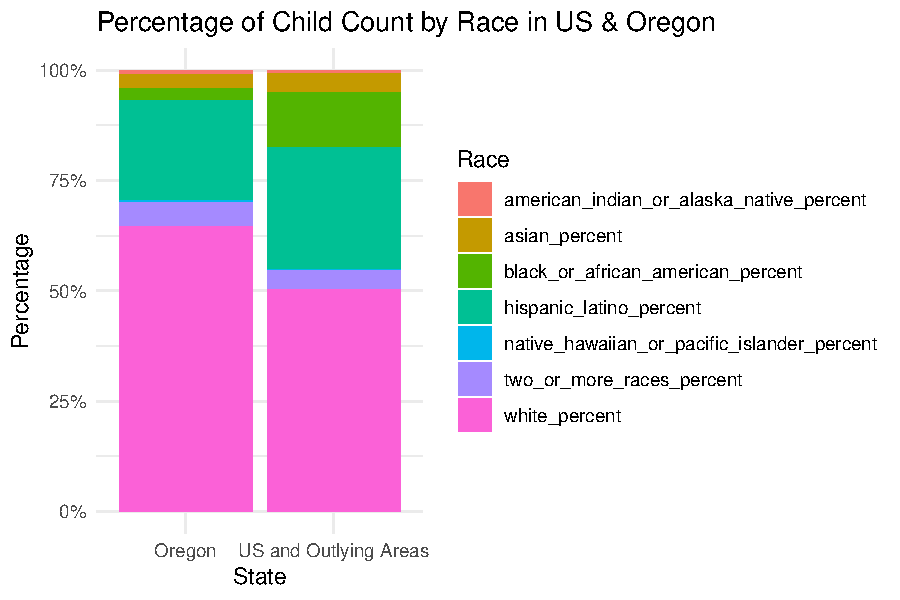
\includegraphics[keepaspectratio]{v2_race_files/figure-pdf/B2-2 Chart 1 without viridis_d-1.pdf}}

\pandocbounded{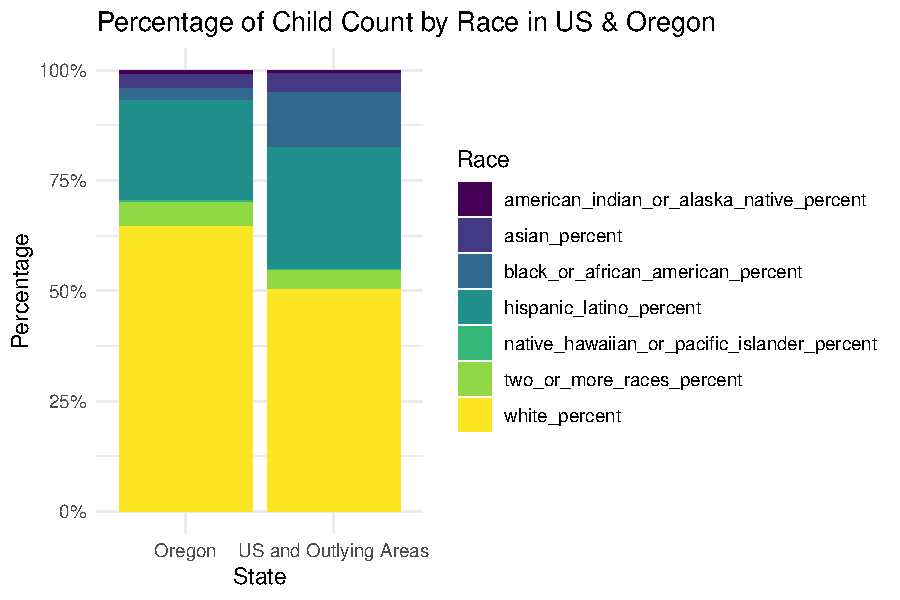
\includegraphics[keepaspectratio]{v2_race_files/figure-pdf/B2-2- v.1 with viridis_d-1.pdf}}

B2 Visualization 2 v.2 - it has labels on the bar but it's ugly as hell

\pandocbounded{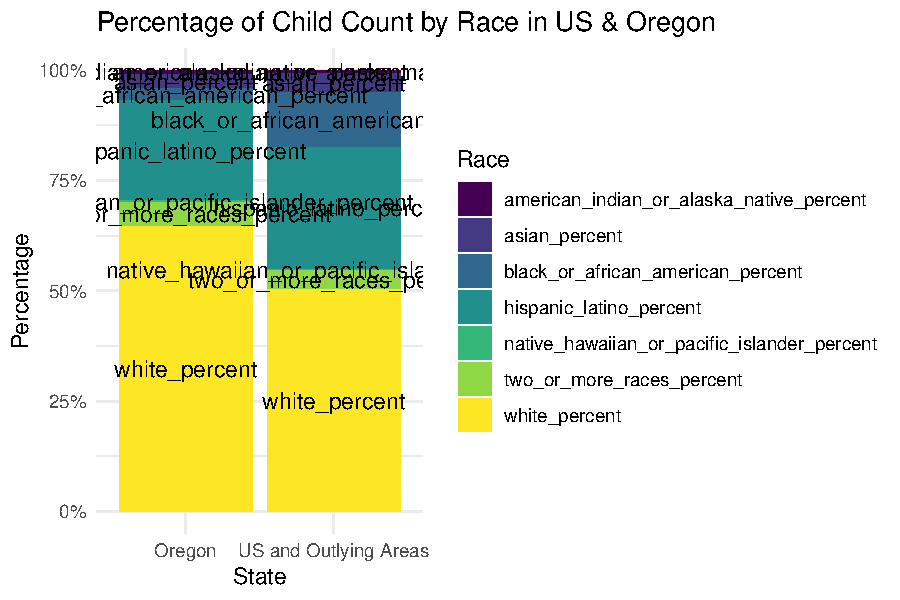
\includegraphics[keepaspectratio]{v2_race_files/figure-pdf/B2-2 v.2 with viridis_d-1.pdf}}

\pandocbounded{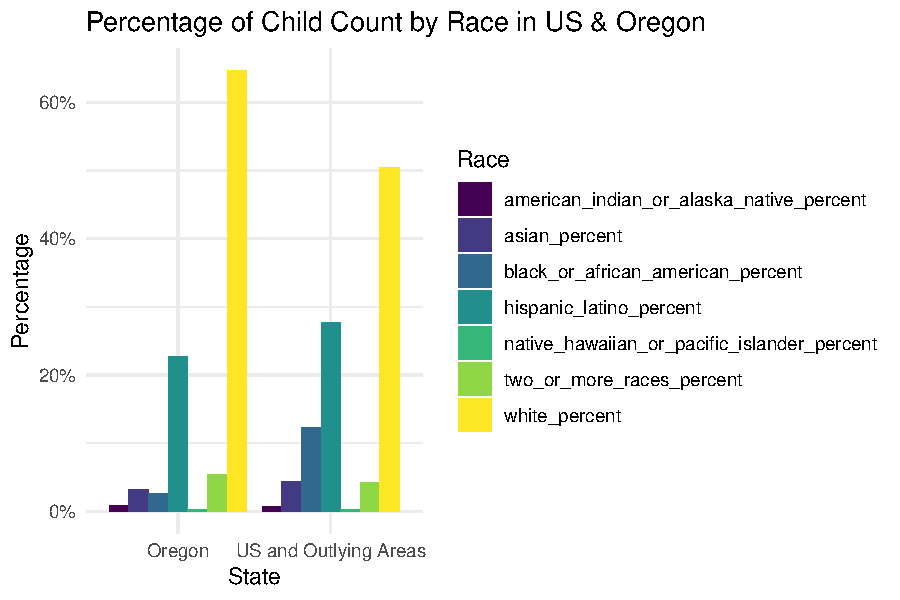
\includegraphics[keepaspectratio]{v2_race_files/figure-pdf/B2-2 v.2 changed it to the bar chart-1.pdf}}

\pandocbounded{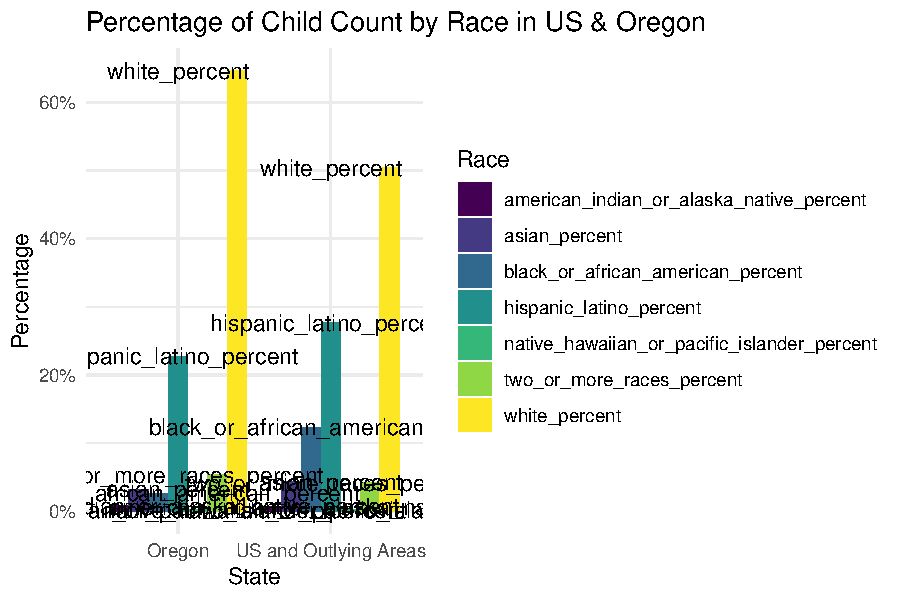
\includegraphics[keepaspectratio]{v2_race_files/figure-pdf/B2-2 v.2 changed to the bar chart AND THEN ADDED LABELS...??-1.pdf}}

\pandocbounded{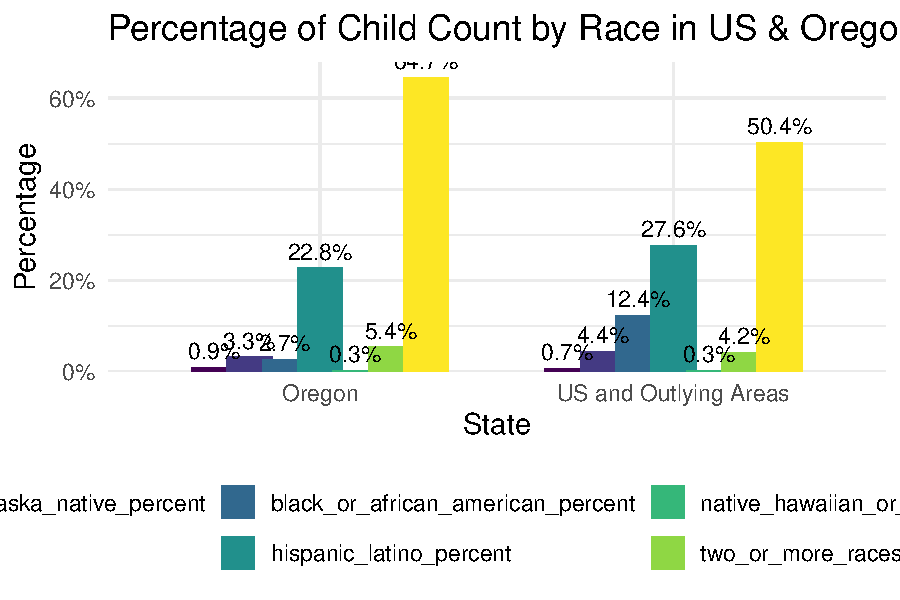
\includegraphics[keepaspectratio]{v2_race_files/figure-pdf/B2-2 v.2 ChatGPT suggsetion-1.pdf}}

\pandocbounded{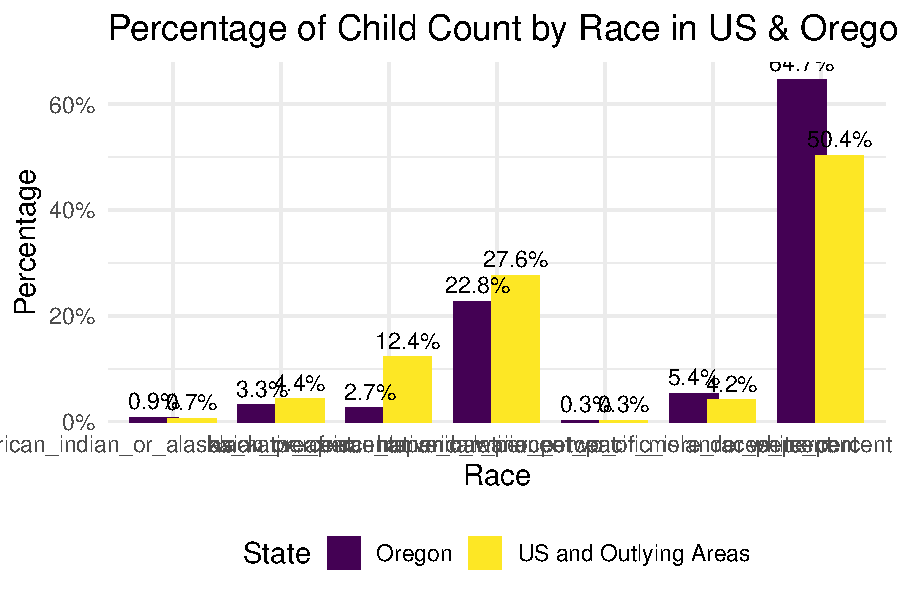
\includegraphics[keepaspectratio]{v2_race_files/figure-pdf/B2-2 v.2 bar chart with each of Oregon and US next to each other-1.pdf}}

\pandocbounded{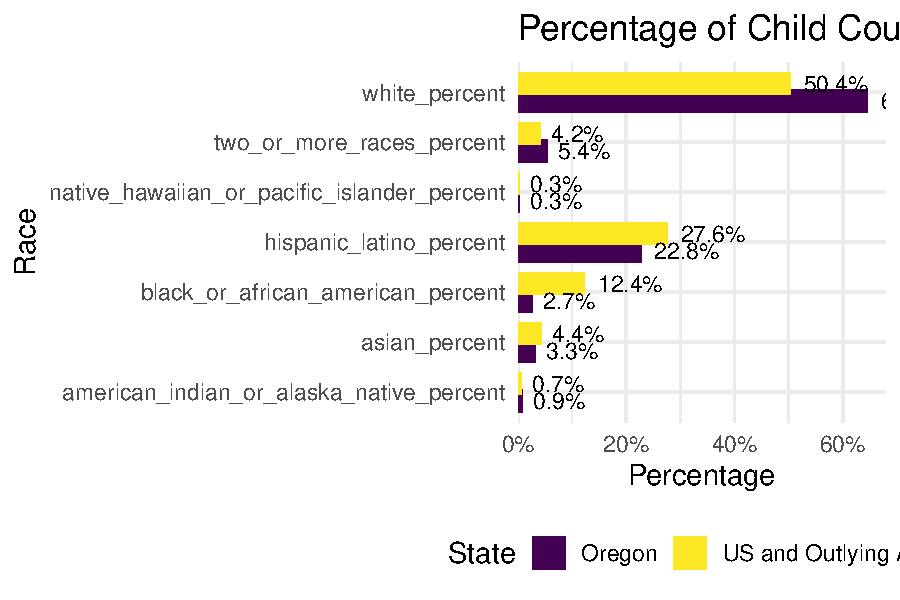
\includegraphics[keepaspectratio]{v2_race_files/figure-pdf/B2-2 v.2 flip the X and Y for readability-1.pdf}}

C. National and Oregon EXIT data by RACE

I FIXED THE MISSING COLUMN by adding back
part\_b\_eligibility\_not\_determined. I think this is what I can use
for CHI-SQUARE WITH RESIDUALS?

I should be able to export df to excel this way but haven't tried it
yet.

agg\_by\_race\_and\_state

OH NO where did Part B eligibility not determined go?!?!?

I'm trying out to see if I can do the chi-square with residuals (per
\url{https://chatgpt.com/share/67a1833d-9fc4-8012-8193-b6fc358a9687})

Chi-square with Residuals 1:

R doesn't like spaces or dashes / - that's why we did clean names, it
could work but it can be tricky later

Chi-square with Residuals 2:

\begin{verbatim}

    Pearson's Chi-squared test

data:  race_matrix
X-squared = 88130, df = 36, p-value < 2.2e-16
\end{verbatim}

Chi-square with Residuals 3:

Cameron: Residuals are what we are measuring anyway. If nothing was
happening, what would be the expected values in the cells in the matrix
(so the residuals = differences between expected and what we see) so
it's a raw differences

\begin{verbatim}
                              exit_total withdrawal_by_parent
Alaska Native/American Indian  -2.271421            -1.529332
Asian                           3.969401            16.392776
Black/African American          7.392204           -32.563128
Hispanic/Latino                -2.007889           -44.502779
More than Two Races            -4.250400             5.768394
Pacific Islander                1.568056             1.271574
White                          -2.817433            52.320627
                              attempts_to_contact_unsuccessful
Alaska Native/American Indian                        32.766855
Asian                                               -46.849271
Black/African American                              145.362643
Hispanic/Latino                                      41.042318
More than Two Races                                   9.926835
Pacific Islander                                      5.482329
White                                              -123.606382
                              moved_out_of_state part_b_eligible_exiting_part_c
Alaska Native/American Indian           5.200877                       4.008193
Asian                                  37.157114                       1.334661
Black/African American                 -5.841365                     -30.058085
Hispanic/Latino                       -44.978596                     -21.284323
More than Two Races                    20.190835                       5.754274
Pacific Islander                        8.578719                      -4.113435
White                                  18.873265                      35.792944
                              complete_or_not_eligible
Alaska Native/American Indian                -9.771775
Asian                                       -23.542186
Black/African American                      -82.092145
Hispanic/Latino                             -70.955800
More than Two Races                           1.450087
Pacific Islander                             -6.844091
White                                       129.036997
                              part_b_eligibility_not_determined
Alaska Native/American Indian                        -16.004425
Asian                                                 18.345906
Black/African American                                54.190397
Hispanic/Latino                                      157.395198
More than Two Races                                  -26.019725
Pacific Islander                                       1.420595
White                                               -170.810660
\end{verbatim}

Chi-square with Residuals 4:

Cameron: How can I reverse the order of Y axis (and I should delete the
exit total row too)

Chi-square with Residuals: Viz 1 (HEATMAP)

\pandocbounded{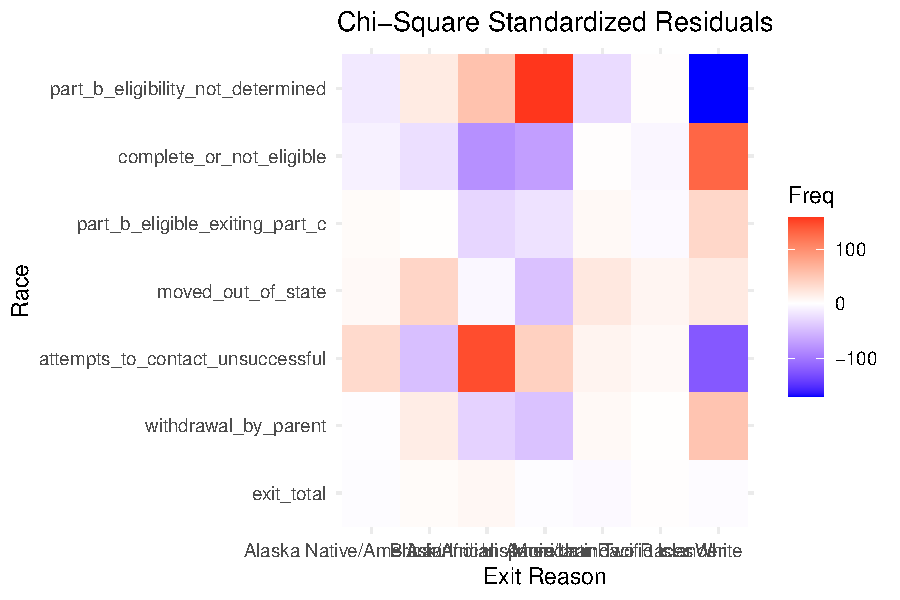
\includegraphics[keepaspectratio]{v2_race_files/figure-pdf/unnamed-chunk-7-1.pdf}}

Chi-square with Residuals: Viz 2 (CORRPLOT:
https://www.sthda.com/english/wiki/chi-square-test-of-independence-in-r\#google\_vignette)

\begin{verbatim}
[1] "exit_total"                        "withdrawal_by_parent"             
[3] "attempts_to_contact_unsuccessful"  "moved_out_of_state"               
[5] "part_b_eligible_exiting_part_c"    "complete_or_not_eligible"         
[7] "part_b_eligibility_not_determined"
\end{verbatim}

corrplot :) Trial 1:
\url{https://cran.r-project.org/web/packages/corrplot/vignettes/corrplot-intro.html}

\pandocbounded{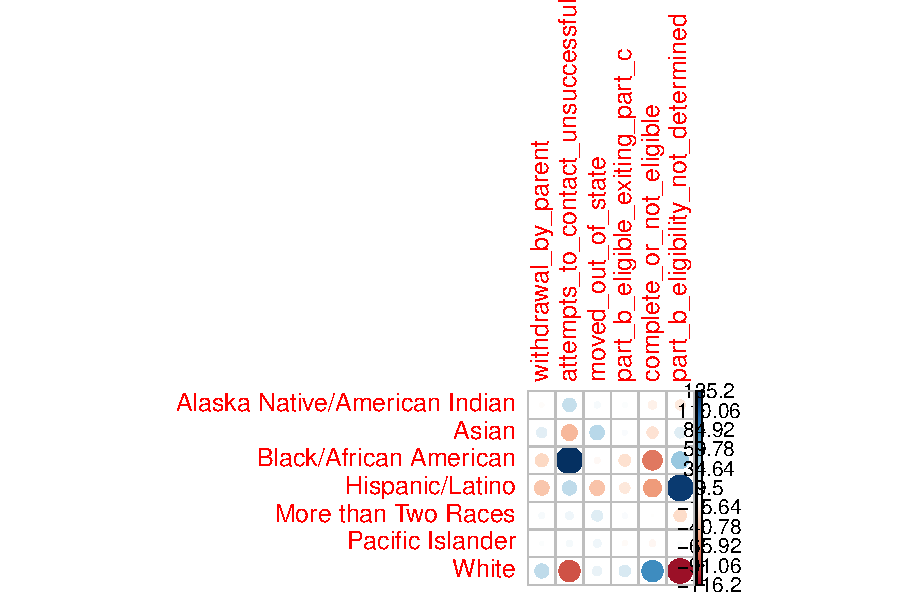
\includegraphics[keepaspectratio]{v2_race_files/figure-pdf/unnamed-chunk-10-1.pdf}}

corrplot trial 2:

\pandocbounded{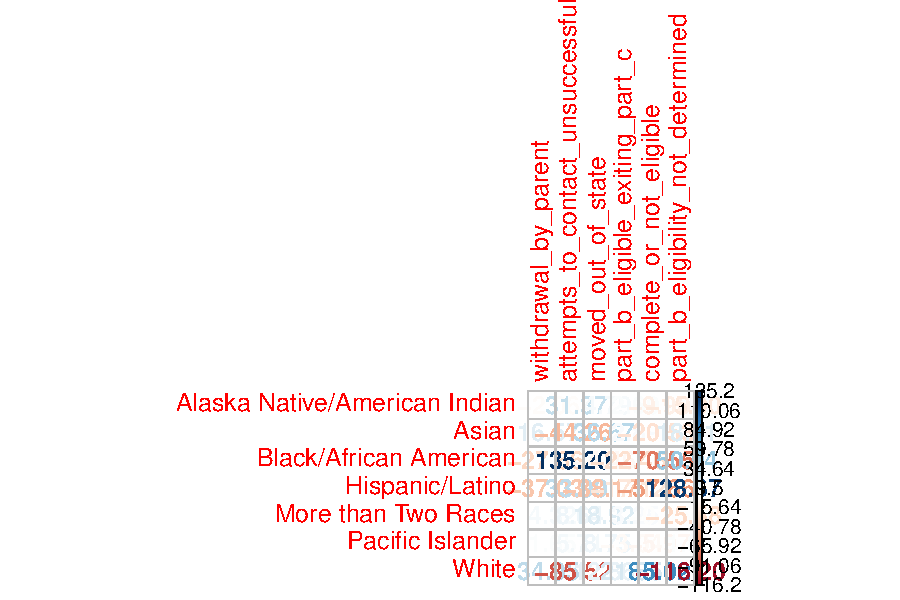
\includegraphics[keepaspectratio]{v2_race_files/figure-pdf/unnamed-chunk-11-1.pdf}}




\end{document}
